\documentclass[11pt]{article}
\usepackage{graphicx}
\usepackage[top=0.75in, bottom=1.75in, left=1in, right=1in,includefoot]
{geometry}
\usepackage{fancyhdr}
\usepackage[colorlinks=true, linkcolor=cyan, citecolor=cyan, urlcolor=blue]{hyperref}
\usepackage{mathpartir}
\usepackage{tikz}
\usetikzlibrary{arrows.meta, positioning}
\usepackage{blindtext}
%remove the line above

\pagestyle{fancy}
\fancyhead[L]{\fancyhdrbox[c]{\Large \slshape \sffamily 
Lambda-Calculi for Logics}}
\fancyhead[C]{}
\fancyhead[R]{\large \sffamily \bfseries Valeria De Paiva }

\fancyfoot[L]{\fancyhdrbox[b]{\sffamily \small Compiled By: \\ 
\normalsize \sffamily Adam Brohl, Ellen Whalen, Vincent Chan}}
%Change the names above to your names

\fancyfoot[C]{\thepage}
\fancyfoot[R]{\fancyhdrbox[b]{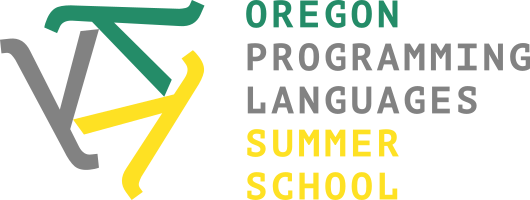
\includegraphics[height=0.35in]{oplssLogo.png}}}
\renewcommand{\footrulewidth}{0.5pt}

\setlength{\parindent}{0pt}
\setlength{\parskip}{2ex}
\setlength{\headheight}{1.25in}

\begin{document}
\thispagestyle{plain}
\begin{center}
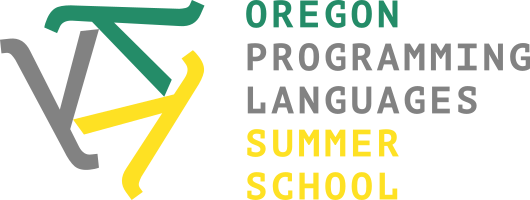
\includegraphics[width=3in]{oplssLogo.png}\\[2\parskip]
\sffamily \LARGE \slshape Lambda-Calculi for Logics
--- \upshape Valeria De Paiva \\[2ex]
\href{https://github.com/vcvpaiva/DialecticaCategories/blob/master/OPLSS2025/OregonLecture1.pdf}{\large Lecture 1 - \slshape June 23, 2025}
\end{center}

\section{History}
At the start of the 20th century (c. 1920-1930), a math revolution took place. Mathematics shifted from a focus on numbers themselves to a focus on algebra and proofs - the structures connecting these numbers. However, it was a ``silent'' revolution since mathematics didn't undergo as explosive of a change as other fields like biology (the theory of evolution) or physics (the quantum revolution). Math is often still perceived as nothing more than its pre-revolution contents, but the concepts introduced in this period of change are incredibly relevant to computing today. Here are some of these relevant concepts:
\begin{itemize}
    \item Category theory 
        \begin{itemize}
            \item further organizes how concepts and structures relate to one another
        \end{itemize}
    \item Curry-Howard correspondence precursors
        \begin{itemize}
            \item 1847: Boolean algebras
            \item 1920: Schonfinkel conbinatory logic
            \item 1945: Kleene realizability
        \end{itemize}
\end{itemize}
\begin{center}
\begin{tikzpicture}[node distance=1.5cm, font=\small]
  \node (lambda) at (90:3) {Church $\lambda$-Calculus};
  \node (ccc) at (210:3) {Cartesian Closed Category};
  \node (logic) at (330:3) {Intuitionistic Prop. Logic};
  \draw[-] (lambda) -- (logic) node[right] {};
  \draw[-] (logic) -- (ccc) node[below] {};
  \draw[-] (ccc) -- (lambda) node[left] {};
\end{tikzpicture}
\end{center}
The Curry-Howard correspondence links logics, programming languages and categories. (Initially, it only connected logics and programming languages.) It came about because Hilbert wished to formalize consistency of arithmetic using finitistic methods in such a manner that the formalism was
\begin{enumerate}
    \item Consistent - no contradictions
    \item Complete - all true statements are provable
    \item Conservative - results about ``real'' objects don't need to rely on ``ideal'' objects
    \item Decidable - statements can actually be shown to be T or F
\end{enumerate}
Gödel's Incompleteness Theorems (1931) showed that this list was not possible with current methods. Gentzen, Hilbert's student, sought to find more powerful methods. Some mathematical highlights of this wartime period include:
\begin{itemize}
    \item Gödel (1933, 1942, 1958) created a liberalized version of Hilbert's program to justify classical systems as intuitively as possible.
    \item Gentzen invented systems of natural deduction and sequent calculus to prove consistency of arithmetic
    \item Church's lambda calculus (1936) and Church Thesis that $\lambda$-definability, recursive functions, and Turing machines are equivalent
\end{itemize}
\noindent\textbf{Curry-Howard for Implication}
\begin{itemize}
\item We connect proofs and programs by using the Curry-Howard correspondence:
\item Natural deduction without $\lambda$-term
    \begin{mathpar}
        \infer{A \to B \\ A}{B}\and
        \infer
        {
            [A] \\\\
            \vdots \pi \\\\
            B
        }
        {A \to B}
    \end{mathpar}
\item Natural deduction with $\lambda$-term
    \begin{mathpar}
        \infer{M\ :\ A \to B \\ N\ :\ A}{M(N)\ :\ B}\and
        \infer
        {
            [x\ :\ A] \\\\
            \vdots \pi \\\\
            M\ :\ B
        }
        {\lambda x:A.\ M\ :\ A \to B}
    \end{mathpar}
\end{itemize}
This led to lambda calculus as a universal programming language, which in turn led to new logics and constructs to extend it. Category theory is helpful for finding and reasoning about these extensions.
\section{Category theory}
Category theory is the general mathematical theory of structures and systems.
\begin{itemize}
    \item \textbf{Types:} formulae/objects in a category
    \item \textbf{Terms/programs:} proofs/morphisms in an \textit{appropriate} category (the appropriate part is the hard part)
    \item \textbf{Category:} collection of objects \& morphisms, where morphisms are arrows between objects that satisfy identity and associativity properties
    \item \textbf{Functor:} morphisms between categories
    \item \textbf{Natural transformation:} morphisms between functors
    \item \textbf{Reduction is proof normalization} (Tait)
\end{itemize}
Why categories? 
\begin{itemize}
    \item Prioritizes modeling derivations rather than truth/falsity - these derivations are useful in many fields (linguistics, functional programming, compilers)
    \item Allows you to solve a problem where it's easier, then transport the solution
    \item Can be used with many different logics:
        \begin{itemize}
            \item System F
            \item Classical logic
            \item Intuitionistic logic
            \item Linear logic
            \item Dependent type theory
            \item Modal logic
            \item High-order logic, etc.
        \end{itemize}
\end{itemize}
\end{document}
